\section{Ergebnisse und Diskussion}

%\begin{figure}[t]
%	\centering
%	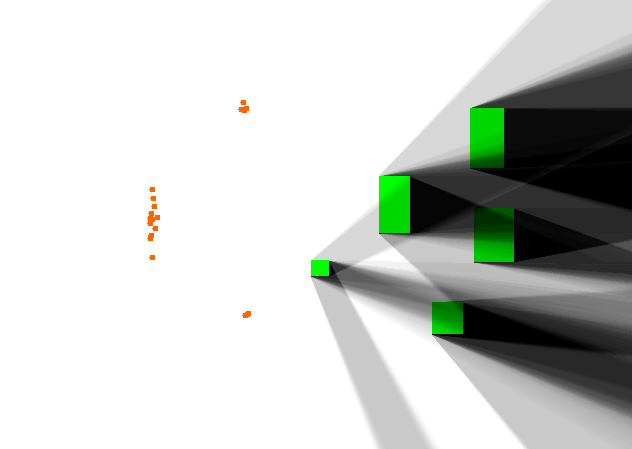
\includegraphics[width=\columnwidth]{images/ergebnis_4.png}
%	\caption{Ergebnis 1}
%	\label{fig:ergeb1}
%\end{figure}

%\begin{figure}[t]
%	\centering
%	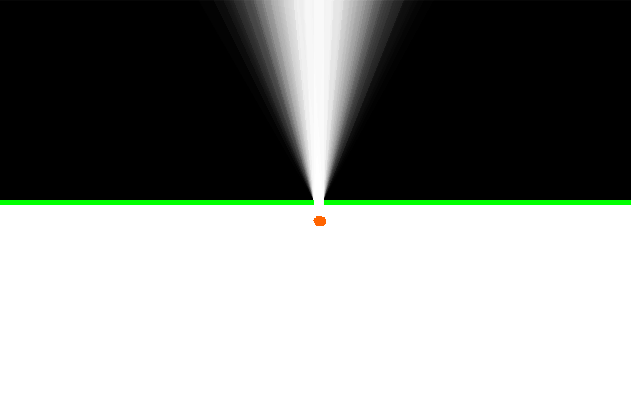
\includegraphics[width=\columnwidth]{images/ergebnis.png}
%	\caption{Ergebnis 2}
%	\label{fig:ergeb2}
%\end{figure}

%\begin{figure}[t]
%	\centering
%	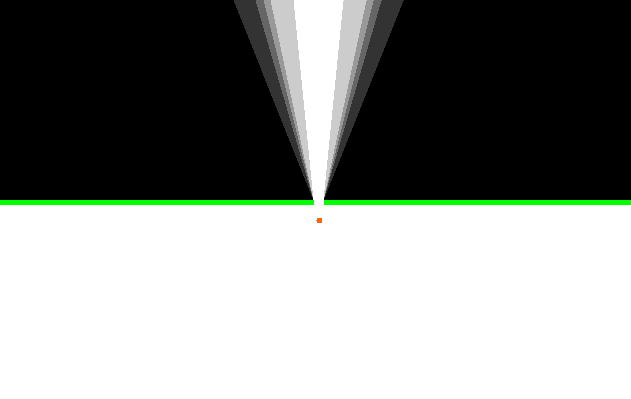
\includegraphics[width=\columnwidth]{images/ergebnis_2.png}
%	\caption{Ergebnis 3}
%	\label{fig:ergeb3}
%\end{figure}

%\begin{figure}[t]
%	\centering
%	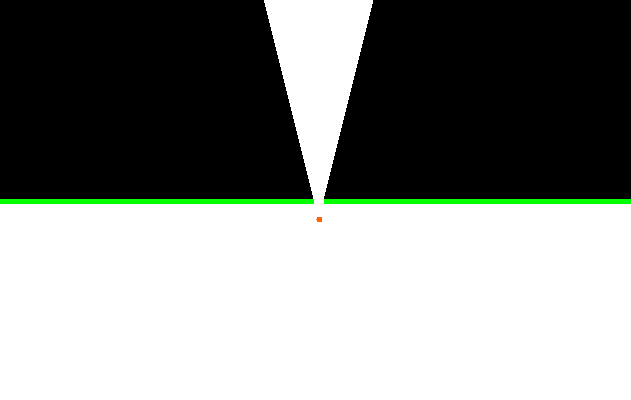
\includegraphics[width=\columnwidth]{images/ergebnis_3.png}
%	\caption{Ergebnis 4}
%	\label{fig:ergeb4}
%\end{figure}

Was Sie hier finden sollten, findet sich leider schon in den vorangegangenen
Textpassagen und Abschnitten und ich mag Sie nicht mit Wiederholungen
langweilen. Jedoch kann man ab und zu feststellen, dass das Abstract und
die Diskussionen eine gewisse Ähnlichkeit aufweisen, wobei die Diskussion
immer ausführlicher sein soll. Das liegt mitunter daran, dass beide
Abschnitte Zusammenfassungen mit unterschiedlicher Nuancierung darstellen.

Jetzt möchte ich mich gleich auf genau dieses Schreiben beziehen,
von dem ich hoffe, dass Sie hinsichtlich des Schreibens und Lesens
von solchen Ideen- und Gedankenmanifestationen etwas für sich mitnehmen konnten.
Selber hatte ich mit diesem Thema verstärkt während meiner Doktorarbeit \cite{Gerhards2008}
zu tun gehabt, ohne selber der enthusiastischste Leser gewesen zu sein.
Viele Ideen und Ansichten habe ich jedoch von meinem Doktorvater
Prof. Dr. Kurt Roth mitbekommen, dessen arbeitsgruppeninterne Übungen
zum schnellen Lesen förderlich für die Adrenalinproduktion waren.

% Ziel der Vorlesung war neben der sehr theorielastigen Einführung
% in die Fourier-Transformation, Faltung, Korrelationsanalyse und
% der nichtlinearen Optimierung, dass Sie sich mit einem Problem
% mit stark physikalischem Schwerpunkt auseinandersetzen sollten.
% Hier galt es sich einzuarbeiten und danach die entsprechenden
% Werkzeuge zum Lösen des Problems sowie zur graphischen Visualisierung
% anzueignen. Die Päsentation sowie der Abschlussbericht stellen
% dann die mündliche, wie schriftliche Darlegung des Problems und
% dessen Lösunng dar.
%
% Und auch wenn Sie mit Ihrem Problem in Zukunft nie wieder in
% Berührung kommen werden, ist es generell wichtig Probleme anzugehen,
% die Werkzeuge zur dessen Bewältigung anzueignen und danach die
% Problemlösung auch voranzutreiben. Wissenschaftlichkeit in den
% Sachverhalt einfließen zu lassen, bedeutet dann noch das Problem
% in einem größeren Kontext zu sehen oder auch in Bezug auf verwandte
% Problematiken.

% Zum Abschluss aber noch einen Witz: Stellen Sie sich eine Party
% vieler mathematischer Funktionen vor. Auf einmal öffnet sich die
% Tür und ein Differentialoperator tritt herein. Alle Funktionen
% suchen die Flucht, nur die e-Funktion bleibt an der Bar stehen.
% Kommt der Differentialoperator zur e-Funktion und fragt, warum
% sie denn nicht weglaufen täte. 'Na, ich bin doch die Funktion e hoch x.
% Du kannst mich nicht wegdifferenzieren.' Darauf antwortet der
% Differentialoperator: 'Aber ich leite doch nach y ab.'

Schließen möchte ich mit einem Zitat von Wittgenstein \cite{Wittgenstein1922},
welches Prof. Dr. Kurt Roth im Zusammenhang wissenschaftlichen
Schreibens gerne nutzte: {\it Was sich überhaupt sagen lässt, lässt
sich klar sagen; und wovon man nicht reden kann, darüber muss man
schweigen.} 
